\chapter{System Model}
\label{chp:system-model}
This chapter elaborates on the modeling aspects of the system being simulated. Having accurate models for both RF and Optical channels is essential for ensuring the reliability and performance of the simulation. These models provide a foundation for understanding and optimizing the system's behavior under various conditions.
\section{High level overview}
The handover algorithm proposed in Chapter \ref{chp:problem_statement} is designed for hybrid networks consisting of a traditional RF transmitter and an optical system utilizing narrow beams for transmission. Appropriate channel models for both media are crucial as they provide the inputs for the proposed handover algorithm, as detailed in Section \ref{subsec:algo-input}. For the RF component, a WiFi model utilizing general industry-standard transmitter and receiver components is considered, maintaining consistency with previous work in mobility management for hybrid optical networks, as seen in \cite{wu_novel_2020} and \cite{wu_smart_2020}. The channel model for the optical system requires further elaboration, as a generic standard model for narrow-beam optical wireless systems does not yet exist. The various components of the optical channel model, especially the SINR and data-rate calculation, depend on the specific design of the transmitter and receiver components, and thus, these need to be modeled as well. Finally, an appropriate user mobility model needs to be considered to evaluate the handover algorithm. Figure \ref{fig:mod-high-level} provides a high-level overview of how the independent models interconnect to provide an accurate system model to simulate.
\begin{figure}
    \centering
    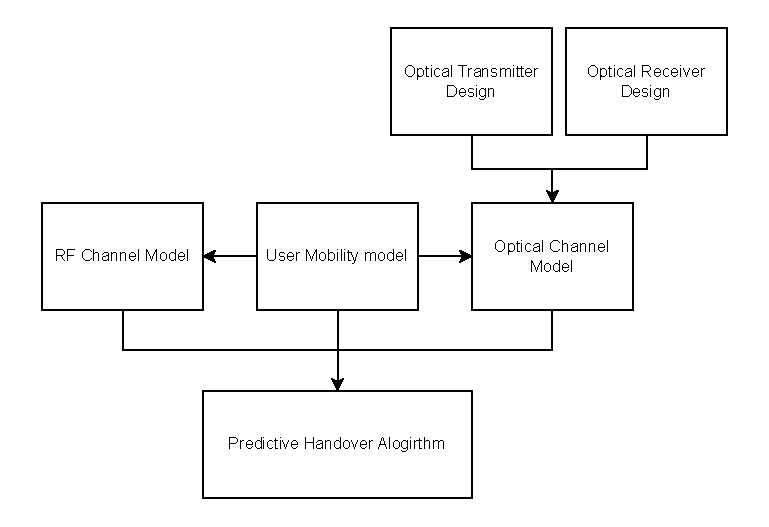
\includegraphics[width=0.75\linewidth]{Figures/modeling-high-level.drawio.pdf}
    \caption{High-level overview of various components being modeled in the simulation}
    \label{fig:mod-high-level}
\end{figure}
\section{RF Network and Channel model}
A Single WiFi AP is placed at the center of the room. To keep inter-cell interference at an undetectable level, the WiFi system employs carrier sense multiple access/collision avoidance (CSMA/CA) similar to the system first presented in \cite{wu_novel_2020-1}.
The Gain of the WiFi AP is given by \cite{perahia_next_2013} as shown below in (\ref{eq:mod-wifi-gain}):
\begin{equation}
    G_{WiFi}^u = |H_{WiFI}^u|^210^{\frac{-L(d_u) + X_\sigma}{10}}.
    \label{eq:mod-wifi-gain}
\end{equation}
Here, $H_{WiFi}^u$ describes the channel transfer function which follows a standard Rayleigh distribution; $X_\sigma$ represents the shadow fading given by a zero-mean Gaussian random variable with a standard deviation of 10dB. Finally $L(.)$ represents the free space path loss as given by \cite{wu_mobility_2018} and shown in (\ref{eq:mod-path-loss}).
\begin{equation}
    L(d) = 
\begin{cases} 
20 \log_{10}(f_c d) - 147.5, & \text{if } d < d_{\text{ref}} \\
20 \log_{10}(f_c d^{2.75} d_{\text{ref}}^{1.75}) - 147.5, & \text{if } d \geq d_{\text{ref}}
\end{cases}.
\label{eq:mod-path-loss}
\end{equation}
Here, $f_c$ represents the central carrier frequency while $d_{ref} = 10 \text{m}$ is the reference distance. Based on these quantities defined above, \cite{wu_mobility_2018} provides the calculation of SNR of a WiFi user given by (\ref{eq:mod-wifi-snr}):
\begin{equation}
    \gamma_{u}^{\text{WiFi}} = \frac{G_{u}^{\text{WiFi}} P^{\text{WiFi}}}{N^{\text{WiFi}} B^{\text{WiFi}}} .
    \label{eq:mod-wifi-snr}
\end{equation}
Here, the PSD of the noise at the receiver is represented by $N_{WiFi}$ while $B_{WiFi}$ and $P_{WiFi}$ represent the system bandwidth and the transmit power of WiFi AP respectively. Given the SNR, and based on the Shannon capacity, as shown in \cite{wu_novel_2020-1}, we can calculate the Capacity of the WiFi Channel as shown in (\ref{eq:mod-wifi-cap}):
\begin{equation}
    r_u = B \log_2(1 + \gamma_{WiFi}^u).
    \label{eq:mod-wifi-cap}
\end{equation}
Figure \ref{fig:mod-rf-model} provides a summary of the various components of the RF model and their relations and dependencies.
\begin{figure}
    \centering
    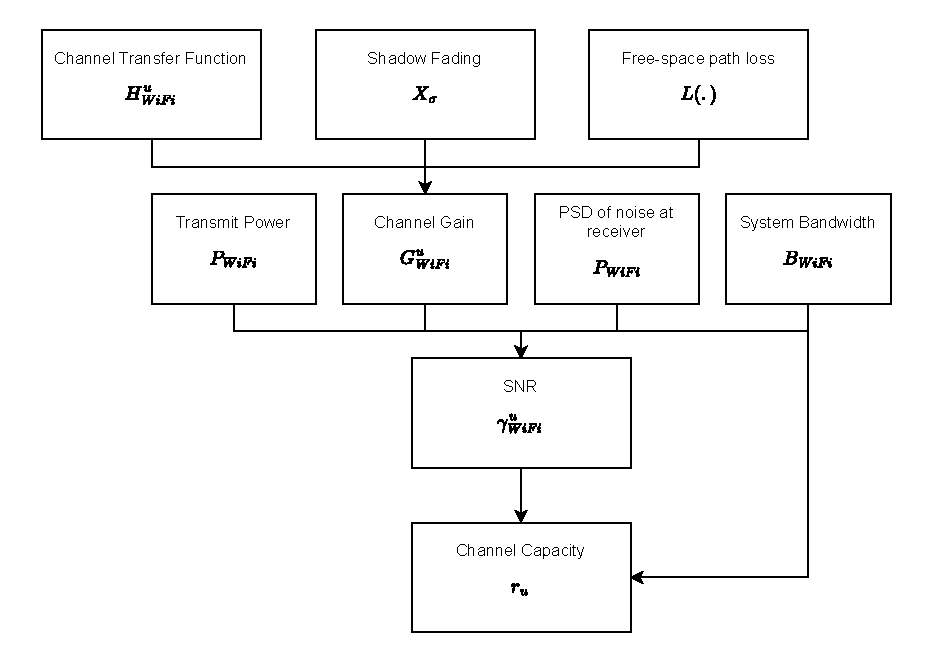
\includegraphics[width=0.75\linewidth]{Figures/RF-channel-model.drawio.pdf}
    \caption{Various components of the RF model and their relations}
    \label{fig:mod-rf-model}
\end{figure}
\section{Optical Network and Channel model}
\section{Optical Transmitter Design}
\section{Optical Receiver Design}
\section{User Mobility model}
User mobility is usually modeled based on popular stochastic models such as the Manhattan mobility model, Reference point group mobility model \cite{kahn_experimental_1995} and the Random Waypoint Model (RWP) \cite{imielinski_dynamic_1996}. The RWP is a popular model widely utilized in the study of mobile ad hoc networks (MANETs) to simulate the movement patterns of mobile nodes. This model operates by having each node pause for a random period at a given location before selecting a new random destination within the simulation area. The node then travels towards this destination at a randomly chosen speed, which is uniformly distributed between a predefined minimum and maximum value. Upon reaching the destination, the node pauses again before repeating the process. This model is characterized by its simplicity and the ability to generate diverse mobility patterns. The original scenario for RWP model was for large outdoor settings with altering speeds when arriving at each waypoint. When adapting the model for indoor scenarios based on changes made by \cite{wu_smart_2020}, where the distance between waypoints is relatively short, the speed is considered to be constant for a short period. The movement within this period is considered an \textit{excursion}. Upon concluding the current excursion, the user selects a new speed, entirely uninfluenced by prior movements, and proceeds to continue traveling. Let $v$ denote the average speed. We assume the user's speed to be uniformly distributed between $0$ and $2v$. Figure \ref{fig:mod-user-mob} shows an example trace of the user movement on the simulator using RWP.
\begin{figure}
    \centering
    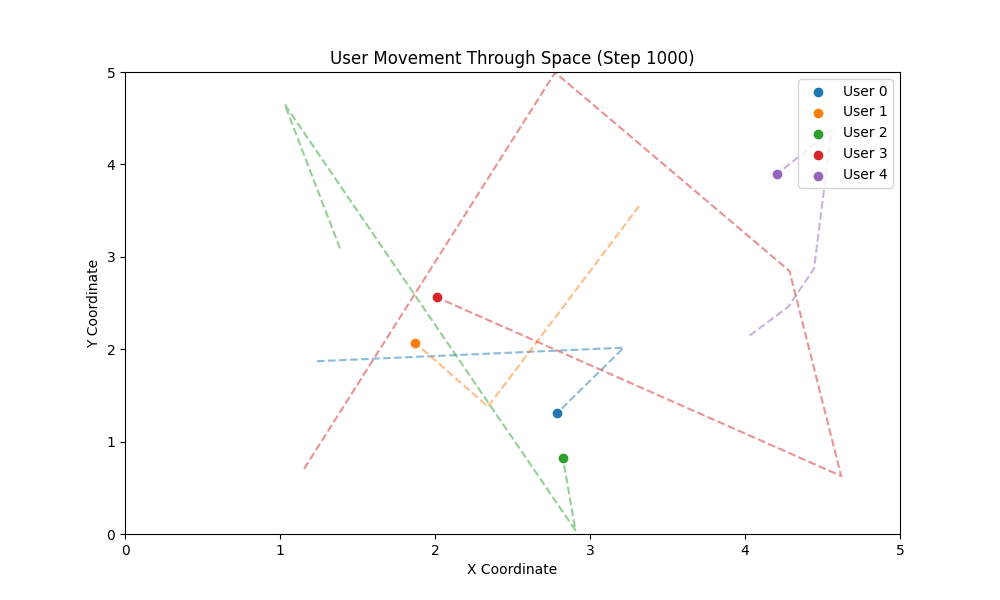
\includegraphics[width=1\linewidth]{Figures/mobility-plot-2025-04-28-15-30-46.png}
    \caption{User mobility simulation based on the RWP}
    \label{fig:mod-user-mob}
\end{figure}
\section{User localization}
\label{sec:mod-user-loc}
User localization is an essential pre-condition for a mobility-aware handover algorithm to operate effectively. The localization strategy varies based on the receiver and transmitter designs and the components used in the hybrid network. However, the handover algorithm itself is not intrinsically coupled to a specific strategy. The algorithm treats localization as a black box from which it extracts the data it deems necessary for evaluation. As such, the handover algorithm can operate with any localization technique that satisfies the following criteria:
\begin{itemize}
    \item \textbf{Location accuracy:} The localization technique should provide accurate location information relative to the coverage area of an individual optical beam. The target is for the location estimation to be accurate enough for the algorithm to identify the individual optical beam that the user can be served by. For example, in our case with the transmitter design considerations, as the coverage area of an individual optical beam is $< 10 \text{cm}$, the localization strategy should be accurate enough in the cm scale.
    \item \textbf{Periodicity of measurements:} As further elaborated in \ref{chp:problem_statement}, the algorithm requires velocity and acceleration information for the decision making process. If this information is being derived from the localization strategy itself, it is critical that the periodicity of the location estimation be frequent enough such that the derived quantities are accurate and up to date
\end{itemize}
Positioning techniques for indoor localization based on RF such as WiFi, Bluetooth and Radio Frequency Identification (RFID) are not suitable candidates due to their low accuracy, high latency and hardware costs\cite{lin_real-time_2020}. Visible Light Positioning (VLP) has become significantly more attractive in this domain due to their low costs and high positioning accuracy. Studies have shown positional accuracy on the centimeter level\cite{hassan_indoor_2015}\cite{xu_experimental_2018}. Based on the receiving device these positioning systems can be divided into two broad categories:
\begin{itemize}
    \item \textbf{Photo-diode based:} Low latency but sensitive to device rotation; positioning accuracy falls where UE does not have a fixed orientation
    \item \textbf{Image sensor based:} Robust to device rotation but real time performance limited. High computational load of image processing or communication latency due to transmission to server.
\end{itemize}
Taking in consideration the transmitter-receiver design as well the requirements of the handover algorithm itself, We decided to utilize a passive beam selection based strategy first proposed in \cite{zeng_vcsel_2022}. The beam selection system utilizing Corner Cube Reflectors (CCR) offers low power consumption and virtually no delay, enabling real-time tracking for high-speed users.
\subsection{Localization based on passive beam selection}
\label{subsec:mod-loc-pas-beam}
The VCSEL array system proposed by Zeng et al. in \cite{zeng_vcsel_2022} employs the signal strength strategy (SSS), which selects the optical beam with the highest received power. Each optical beam provides coverage to a specific area on the receiver plane. Thus, by considering the 3 optical beams with the highest received power, we can use triangulation to estimate the location of the user. The selection of the index of the beams to be utilized for this purpose can be formalized by (\ref{eq:mod-loc-1})
\begin{equation}
    \{I_1, I_2, I_3\} = \arg \max_{n \in N} \{{P_{rx,UE}^n}\}_{\text{top 3}}.
    \label{eq:mod-loc-1}
\end{equation}
Where \(I\) represents the index of the optical beam, \(N\) denotes the set of beams, and \(P_{r_{x,UE}}^n\) signifies the received optical power from the \(n\)-th beam. The strategy utilizes CCR to obtain a power matrix and then find the serving beam. Each VCSEL is associated with an RX element which detects any Reflected Signals (RS) associated with the user. Figure \ref{fig:mod-loc-ap} showcases the AP setup with the RX element associated with each VCSEL.
\begin{figure}
    \centering
    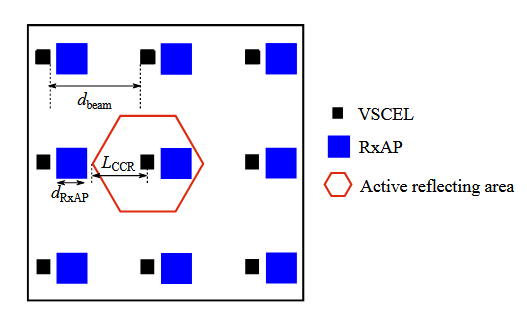
\includegraphics[width=0.75\linewidth]{Figures/modeling-localization-ap-design.png}
    \caption{The setup of AP using a CCR\cite{zeng_vcsel_2022}}
    \label{fig:mod-loc-ap}
\end{figure}

All beams send out a test signal simultaneously every set period. The UE sends back an (RS) which is received by the RxAPs. The optical beam selection is done according to (\ref{eq:mod-loc-1}), Based on which location information is estimated. If the user is not connected to any optical beam, the optical beam with the highest power establishes connection and begins data transmission. Figure () provides an example of this operation in a system with 5 beams. 
\begin{figure}
    \centering
    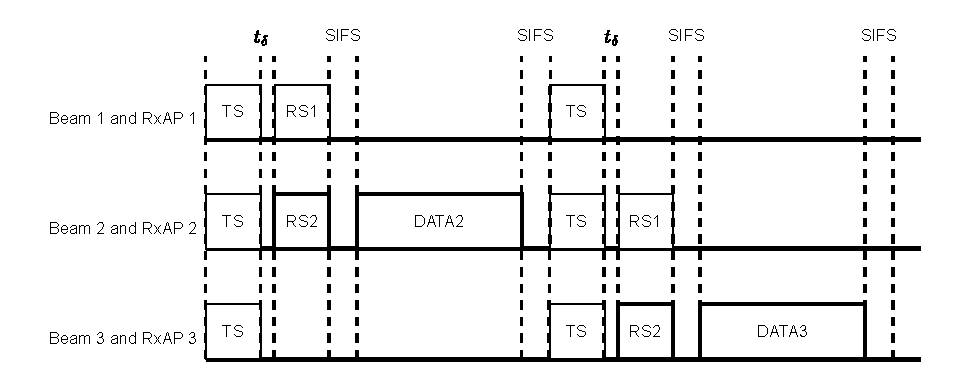
\includegraphics[width=\linewidth]{Figures/RF-OW-modeling-User localization.drawio.pdf}
    \caption{Beam selection mechanism}
    \label{fig:mod-loc-beam-ac}
\end{figure}
In the first period, All beams send a Test Signal (TS). The UE responds with a RS after a mean propagation delay of $t_\delta$. The optical beams for triangulation are first selected. The optical beam with the highest power (in this case beam 2) then starts transmission after a Short Inter-Frame Space (SIFS). In the second period, again all the beams transmit a TS and the location estimation and beam selection procedure repeats (this time selecting beam 3).
The parameters for this selection criteria are shown in Table \ref{tab:mod-loc-params}.
\begin{table}[]
    \centering
    \begin{tabular}{|l|l|l|}
\hline
\textbf{Parameter}            & \textbf{Symbol}   & \textbf{Value}    \\ \hline
Test signal time              & $t_{TS}$          & 0.3 micro-seconds \\ \hline
Reflected signal time         & $t_{RS}$          & 0.3 micro-seconds \\ \hline
Average length of data packet\cite{khorov_tutorial_2019} & $L_{\text{Data}}$ & 64 Kbytes         \\ \hline
Mean propogation delay\cite{higgins_genetic_2009}        & $t_\delta$         & 3 nano-seconds    \\ \hline
SIFS\cite{khorov_tutorial_2019}                         & SIFS              & 2 micro-seconds   \\ \hline
\end{tabular}
    \caption{Parameters for beam selection\cite{zeng_vcsel_2022}}
    \label{tab:mod-loc-params}
\end{table}

The accuracy of this localization strategy was verified by Zeng el al. by simulating a system consisting of 9 VCSELs carried out in Zemax. The results are show in Figure (). Each $L_i$ indicates the position of the user. 